\documentclass[main.tex]{files}
\begin{document}

\chapter{Related Work}
This chapter presents information about known musical notations and some of the most relevant
projects and tools being developed or used.

\section{Musical Notations} 

\subsection{Abc}

Most music notation programs have a visual approach in which the user drags and drops notes
and symbols using the mouse, and the resulting sheet is displayed on the screen. An alternative
approach is writing music using a text-based notation. This is a non-visual mode that represents
notes and other symbols using \ac{ASCII} characters making it economic and intuitive to use and
also making for faster transcriptions. A specialized program then translates the notation into
printable sheet music in some electronic format (e.g. in PDF) and/or into a MIDI file.

Many text-based notations have been invented, and one of them was Abc\cite{abcnotation:Online},
introduced by Chris Walshaw in 1991 as a means to share traditional folk music such as Irish jigs.
Abc is a musical notation standard and not a software package. Abc was later expanded to provide
multiple voices (polyphony), page layout details, and MIDI commands. This was called Abc 2.1.

An Abc tune consists of a header which provides fields for title, composer, key signature,
time signature and default note duration. The music is notated using the letters A to G to
represent the notes.\\
This language has a simple and clean syntax, and is powerful enough to
produce professional and complete music scores. Among other advantages, the following are the
most important: 
\begin{itemize}
  \item powerful enough to describe most music scores available in paper; 
  \item actively maintained and developed; 
  \item the source files are written in plain text files; 
  \item easy searching and indexing of tune books and easy creation of music archives; 
  \item there are already many tools for transforming and publishing; 
  \item this format can be easily converted to other known formats; 
  \item compact and clear notation; 
  \item human readable;
  \item thousands of tunes available on the Internet; 
  \item open source.
\end{itemize}

This thesis focus on this notation mainly because it appeared as a necessity to study the
feasibility of using automated tests over Abc documents in the context of WikiScore.

The state of the art of Abc is currently represented by two programs: the abcm2ps typesetter,
and the MIDI creator abc2midi. Both are free software released under the GNU GPL license.

Figure \ref{fig:abc_example} is an example of a source file written in Abc and an illustration of
the image generated.

\begin{figure}[htb]
  \centering 
  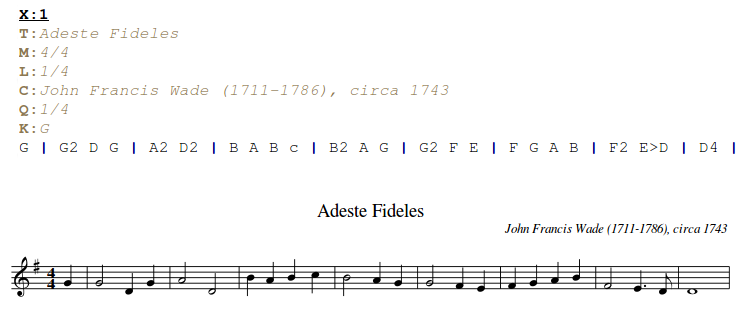
\includegraphics[width=0.8\textwidth]{img/adeste_abc.png} 
  \caption{Abc Notation Example - Excerpt of Adeste Fideles}
  \label{fig:abc_example}
\end{figure}
% 
% \begin{figure}[htb]
%   \centering 
%   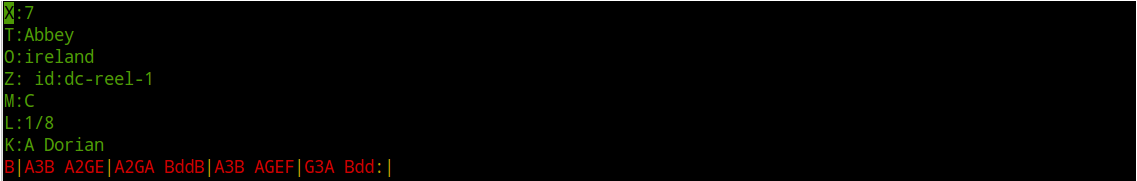
\includegraphics[width=0.8\textwidth]{img/abbey_abc.png} 
%   \caption{Abc Notation Example}
%   \label{fig:abc_example}
% \end{figure}
% 
% \begin{figure}[htb]
%   \centering 
%   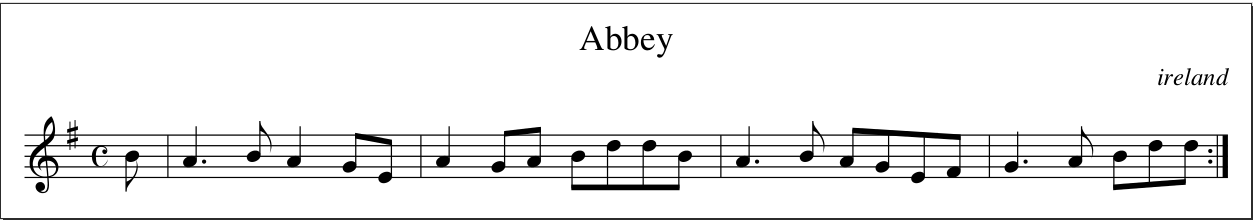
\includegraphics[width=0.8\textwidth]{img/abbey.png} 
%   \caption{Image generated from notation example in Figure \ref{fig:abc_example}1} 
%   \label{fig:abc_example_generated}
% \end{figure} 
% \newpage

\subsection{LilyPond}

GNU LilyPond\cite{lilypond:Online} is a computer program and file format for music engraving. It
formats music beautifully and automatically, and has a friendly syntax for its input files. It is
Free Software (‘open source’). One of LilyPond's major goals is to produce scores that are engraved
with traditional layout rules, reflecting the era when scores were engraved by hand.

Although there are some small similarities to the Abc notation, there are significant differences,
starting with intent. The original intent of the Abc notation was to create a simple means of
sharing folk tunes that could be read as text and sent as email. The Abc notation is a standard, not
software. LilyPond is a software with the intent of creating printed musical scores that match the
best hand engraved musical scores of the past.

The similarity between Abc notation and the LilyPond software is that the basic means of specifying
the notes in a musical score is by using plain text source files and the characters 'a' to 'g' to
represent musical notes.

LilyPond has a much more ambitious goal than Abc notation and the markup language for the LilyPond
source file can become complex quickly if the goal is to combine melody, tab, chords, chord diagrams
and lyrics.

Figure \ref{fig:lilypond_example} is an example of a source file written in LilyPond and an
illustration of the image generated.
% Figure \ref{fig:lilypond_example} is an example of a source file written in LilyPond. Figure
% \ref{fig:lilypond_example_generated} illustrates the image generated using the source illustrated
% in Figure \ref{fig:lilypond_example}.

\begin{figure}[htb]
  \centering 
  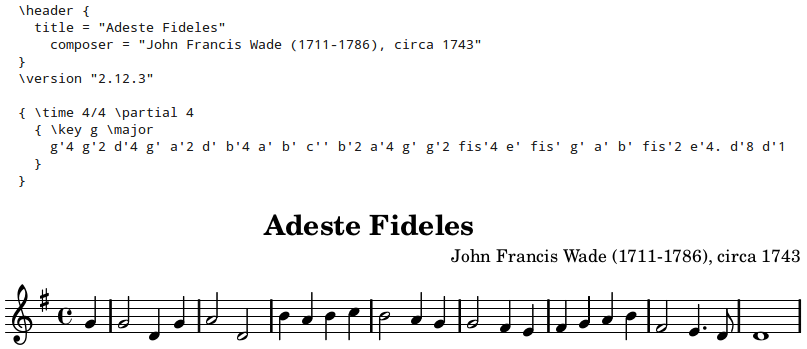
\includegraphics[width=0.8\textwidth]{img/adeste_ly.png} 
  \caption{LilyPond Example - Excerpt of Adeste Fideles} 
  \label{fig:lilypond_example}
\end{figure}

% \begin{figure}[htb]
%   \centering 
%   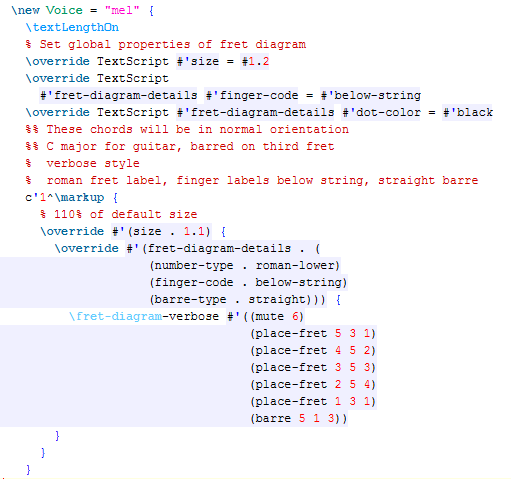
\includegraphics[width=0.8\textwidth]{img/markup-chord-ly1.png} 
%   \caption{LilyPond Chord Diagram Markup} 
%   \label{fig:lilypond_example}
% \end{figure}
% 
% \begin{figure}[htb]
%   \centering 
%   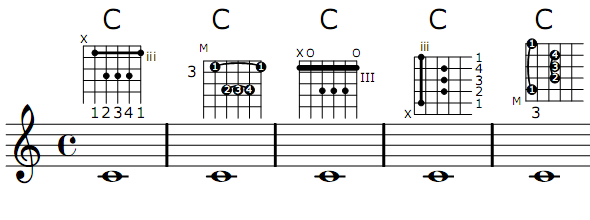
\includegraphics[width=0.8\textwidth]{img/example-chord-diagrams1.png}
%   \caption{Image generated from notation example in Figure \ref{fig:lilypond_example}}
%   \label{fig:lilypond_example_generated}
% \end{figure} 
\newpage

\subsection{MusicXML}

MusicXML\cite{musicxml:Online} is an XML-based file format for representing Western musical notation
designed for notation, analysis, retrieval, and performance applications. The format is proprietary,
developed by Recordare LLC, but fully and openly documented, and can be freely used under a Public
License.

MusicXML was designed from the ground up for sharing sheet music files between applications, and
for archiving sheet music files for use in the future. MusicXML files are readable and usable by a
wide range of music notation applications, now and in the future. MusicXML complements the native
file formats used by Finale and other programs, which are designed for rapid, interactive use.

\section{Projects and Tools} 

This section lists some of the most relevant projects and tools being developed or used at the
moment.

\begin{description}
  \item[\textbf{abcm2ps}]\cite{abcm2ps:Online}
    A command line program which translates tunes written in Abc music notation to customary
    sheet music scores in PostScript or SVG format.
    This is a format related to PDF, and it can be viewed and printed with another free program:
    Ghostscript. This application converts PostScript files into several formats, Acrobat PDF
    being the most important.

    It is based on abc2ps 1.2.5 and was developed mainly to print Baroque organ scores that
    have independent voices played on multiple keyboards and a pedal-board. The  program  has
    since been extended to support various other notation conventions in use for sheet music
    and is now one of the most complete abc implementations.

    It is developed in C language and the author, an organist and programmer called Jean-François
    Moine, releases “stable” and “development” versions of his program. As of this
    writing\footnote{\today}, the stable release is 6.6.22 and the development release is
    7.3.5. Since release 7.2.1 that abcm2ps tries to follow the Abc standard version 2.1.

  \item[\textbf{abc2midi}]\cite{abc2midi:Online}
    A program that converts an abc music notation file to a MIDI file.
    
    It is part of the abcMIDI package, which includes other utility applications.\\ The program
    was developed in C language by James Allwright in the early 1990s and has been supported by
    Seymour Shlien since 2003. The program contains many features, such as expansion of guitar
    chords, drum accompaniment, and support for micro tones, that do not exist in other packages.

  \item[\textbf{EasyAbc}]\cite{easyabc:Online}
    An open source Abc editor for Windows, OSX and Linux.
    
    It uses abcm2ps and abc2midi, and it has a rich feature list. Most notably, it can import
    MusicXML files and export tunes in SVG format. It is published under the GNU Public License
    and was developed by Nils Liberg.

  \item[\textbf{abcpp Preprocessor}]\cite{abcplus:Online}
    A simple yet powerful preprocessor designed for, but not limited to, Abc music files.
    
    It was written to overcome incompatibilities between Abc packages, and to facilitate writing
    portable, and more readable Abc files.\\ 
    A preprocessor is a program that modifies a text file, according to commands contained in the 
    file.
    
    It provides: 
    \begin{itemize}
      \item conditional output; 
      \item exclude or include parts of a piece according to specified conditions; 
      \item define macros, i.e. symbols and sequences of customized commands;
      \item rename commands, symbols, and notes; 
      \item include parts of other files.
    \end{itemize}
    
    One of the usages of this program is the extraction of separate parts from a score.

  \item[\textbf{Abcp}]\cite{abcp:Online}
    A parser for the Abc music notation.
    
    It is a C library that interprets the simple, but very powerful, music notation Abc. It is
    released as open source, under the terms of the BSD license, and may be used in both free and
    commercial software.\\ 
    Abcp has been designed with the following requirements in mind: 
    \begin{itemize}
      \item to be able to handle the Abc 2.0 standard as well as previous standards and the
      extensions introduced by the most widely used tools (abcm2ps, abcmidi, ...); 
      \item to be fast; 
      \item to be small: there must be a fair trade-off between size and functionalities; 
      \item to be easily embeddable: no big restriction on the programming language to use;
      \item to be usable: no complex API or class hierarchy to remember.
    \end{itemize}

  \item[\textbf{Music::Abc::Archive}]\cite{music_abc_archive:Online}
    A Perl module to parse Abc music archives.
    
    Abc music archives contain songs in the Abc format. They are a very quick way for entering
    music in a text format, and there are numerous publishable quality renderers for Abc
    music. This module encapsulates the Abc archive, and individual songs so they may more
    easily be managed by Perl front-ends.

  \item[\textbf{Music21}]\cite{Music21:Online}
    A Python-based toolkit for computer-aided musicology.
    
    Music21 is a set of tools for helping scholars and other active listeners answer questions
    about music quickly and simply.

    Music21 builds on preexisting frameworks and technologies such as Humdrum, MusicXML,
    MuseData, MIDI, and Lilypond, but Music21 uses an object-oriented skeleton that makes it
    easier to handle complex data. But at the same time Music21 tries to keep its code clear
    and make reusing existing code simple.

    Applications of this toolkit include computational musicology, music informations, musical
    example extraction and generation, music notation editing and scripting, and a wide variety
    of approaches to composition, both algorithmic and directly specified.

    It also has a large corpus of musical scores in many formats, including Abc and MusicXML.
\end{description}

\section{Summary}

As said earlier in this chapter the notation that will be used as the basis of this thesis is Abc,
because it is a simple to use but powerful notation. As Wiki::Score was the case study that initially
justified the need for this thesis, it's only logical that Abc is the notation selected.\\
Of course LilyPond, as well as the others notations presented would be a very good alternative. For
that reason, they will not be completely forgotten, as the toolkit might eventually accept other
notations as input/output, making it a more general toolkit as the title of this thesis suggests.

The \textit{de facto} standard programs for Abc are abcm2ps and abc2midi. This fact makes the use of
them almost mandatory or at least serve as inspiration for the tools that will be built, mainly
regarding parsers and internal representations.\\
Nonetheless the other programs may prove valuable pieces of software that, in the same way as the
first two, provide additional features for studying that may be implemented in the toolkit.

\end{document}
